\documentclass[11pt,a4paper]{article}

\usepackage[utf8]{inputenc}
\usepackage[T1]{fontenc}
\usepackage[french]{babel}
\usepackage{times}
\usepackage{graphicx}
\usepackage{amsmath,amssymb}
\usepackage{booktabs}
\usepackage{hyperref}
\usepackage{xcolor}
\usepackage{enumitem}
\usepackage{caption}
\usepackage{float}
\usepackage{geometry}

\geometry{a4paper, left=2cm, right=2cm, top=2cm, bottom=2cm}
\definecolor{darkblue}{RGB}{0,51,102}
\hypersetup{colorlinks=true, linkcolor=darkblue, citecolor=darkblue, urlcolor=darkblue}

\title{\textbf{Pipeline HTR et NLP pour la Transcription Automatique\\de Manuscrits Médiévaux Français (XIII\textsuperscript{e}--XV\textsuperscript{e} siècle)}}
\author{
\textbf{Asmaa OUARAZ} \quad \textbf{Sanaa OUARAZ} \quad \textbf{Ayoub BOUSSLAMA} \quad \textbf{Amine HAMOUMA}\\[0.3cm]
Master Data \& Intelligence Artificielle --- Module Vision par Ordinateur\\
HETIC --- Projet MD5 2026
}
\date{Juin 2026}

\begin{document}
\maketitle

% ============================================================
\begin{abstract}
\noindent
Nous présentons un pipeline end-to-end de traitement automatique de manuscrits médiévaux français, couvrant la reconnaissance de texte manuscrit (HTR, Volet~1) et l'analyse linguistique (NLP, Volet~2). Trois modèles HTR sont comparés sur deux corpus distincts (CREMMA Médiéval et CATMuS+HIMANIS)~: \textbf{Kraken} (CNN+LSTM) atteint un CER de \textbf{6,0\%} (seuil d'excellence) sur CREMMA, tandis que \textbf{TrOCR} adapté par LoRA ($r=8$) atteint \textbf{15,3\%}. Sur le corpus CATMuS+HIMANIS, un second fine-tuning Kraken obtient une accuracy de \textbf{0,79}. Le test de McNemar ($\chi^2=38,25$, $p<0,001$) confirme la supériorité significative de Kraken. Le Volet~2 implémente un module d'expansion des abréviations médiévales (approche séquence-à-séquence), une reconnaissance d'entités nommées (CamemBERT) et une modélisation thématique (BERTopic, 5 topics). Le pipeline intègre la segmentation par SAM et Kraken BLLA, avec export PAGE~XML et contrat de données JSON.

\vspace{0.2cm}
\noindent\textbf{Mots-clés~:} HTR, manuscrits médiévaux, Kraken, TrOCR, LoRA, CREMMA, CATMuS, gothique textualis, SAM, NER, BERTopic, abréviations
\end{abstract}

\vspace{0.5cm}

% ============================================================
\section{Introduction}

La numérisation massive des archives médiévales par des institutions comme la BnF (380\,000 manuscrits, 11 millions de documents en ligne via Gallica) ouvre des perspectives inédites pour la recherche historique. Cependant, une image n'est pas un texte~: la transcription manuelle par des paléographes ($\sim$50\,\texteuro/h) est prohibitivement coûteuse à l'échelle des collections patrimoniales.

La reconnaissance automatique de texte manuscrit (HTR) vise à combler ce fossé. Les manuscrits médiévaux français présentent des défis spécifiques~:
\begin{itemize}[leftmargin=*, itemsep=2pt]
\item \textbf{Variabilité des écritures}~: caroline, textualis, cursiva --- chaque siècle et région a ses particularités
\item \textbf{Abréviations omniprésentes}~: jusqu'à 40\% des mots sont abrégés (tildes nasaux, lettres suscrites, signes tironiens)
\item \textbf{Mélange de langues}~: latin administratif mêlé au moyen français
\item \textbf{Dégradation physique}~: encre effacée, supports endommagés
\end{itemize}

Ce projet se structure en deux volets~: (1)~le \textbf{Volet HTR} produit des transcriptions automatiques à partir d'images de manuscrits, (2)~le \textbf{Volet NLP} analyse ces transcriptions (expansion des abréviations, extraction d'entités, modélisation thématique). Les transcriptions du Volet~1 alimentent directement le Volet~2.

\textbf{Contributions~:}
\begin{enumerate}[leftmargin=*, itemsep=2pt]
\item Un pipeline reproductible end-to-end~: prétraitement $\rightarrow$ segmentation $\rightarrow$ HTR $\rightarrow$ NLP
\item Une comparaison rigoureuse de trois configurations HTR avec test de McNemar
\item Un module d'expansion des abréviations médiévales (séquence-à-séquence)
\item Un CER de 6,0\% (seuil d'excellence) démontrant la faisabilité de l'HTR automatique
\end{enumerate}

% ============================================================
\section{État de l'art}

\subsection{Architectures HTR}

\textbf{Kraken} \cite{kiessling2019} est un système HTR basé sur CNN+LSTM+CTC, moteur de la plateforme eScriptorium. L'encodeur convolutional extrait des features visuelles, le LSTM bidirectionnel modélise les dépendances séquentielles. Kraken est le standard en humanités numériques pour les documents historiques.

\textbf{TrOCR} \cite{li2023} adopte une architecture encoder-decoder Transformer~: un ViT encode l'image, un décodeur GPT-2 génère la transcription token par token. Cette architecture modélise des dépendances contextuelles globales.

\textbf{LoRA} \cite{hu2022} gèle le modèle et n'entraîne que des matrices de faible rang ajoutées aux couches d'attention. Avec $\sim$1\% des paramètres entraînés, LoRA réduit les besoins en mémoire et en données.

\textbf{SAM} \cite{kirillov2023} (Segment Anything Model) est un modèle de segmentation universel pré-entraîné sur 11M d'images. Il peut segmenter n'importe quel objet sans entraînement spécifique.

\subsection{Jeux de données médiévaux}

\textbf{CREMMA Médiéval}~: $\sim$20\,000 lignes, 14 manuscrits français (XIII\textsuperscript{e}--XV\textsuperscript{e} siècle), gothique textualis.

\textbf{CATMuS Medieval}~: $>$160\,000 lignes multilingues, 200 manuscrits (VIII\textsuperscript{e}--XVII\textsuperscript{e} siècle).

\textbf{HIMANIS-Guérin}~: registres de chancellerie royale (XIV\textsuperscript{e} siècle), gothique cursive administrative.

\subsection{Métriques}

Le \textbf{CER} (Character Error Rate) mesure la distance d'édition normalisée au niveau caractère. Le \textbf{WER} opère au niveau mot. Le \textbf{test de McNemar} compare statistiquement deux modèles ligne par ligne.

% ============================================================
\section{Données}

\subsection{Corpus A~: CREMMA Médiéval}

20\,327 lignes extraites de 14 manuscrits littéraires français (XIII\textsuperscript{e}--XV\textsuperscript{e} siècle) en écriture gothique textualis. Genres~: hagiographies (30\%), épopées (17\%), romans (25\%), textes moraux (28\%). Split par manuscrit~: 18\,092 train / 2\,235 validation.

\subsection{Corpus B~: CATMuS + HIMANIS-Guérin}

33\,510 lignes combinant CATMuS Medieval (français) et HIMANIS-Guérin (registres de chancellerie royale, XIV\textsuperscript{e} siècle). Split~: 23\,444 train / 5\,954 val / 4\,112 test.

\subsection{Conventions de transcription}

Transcription graphémique (CATMuS)~: abréviations conservées, pas de normalisation u/v ou i/j, espaces lexicaux.

\begin{figure}[H]
\centering
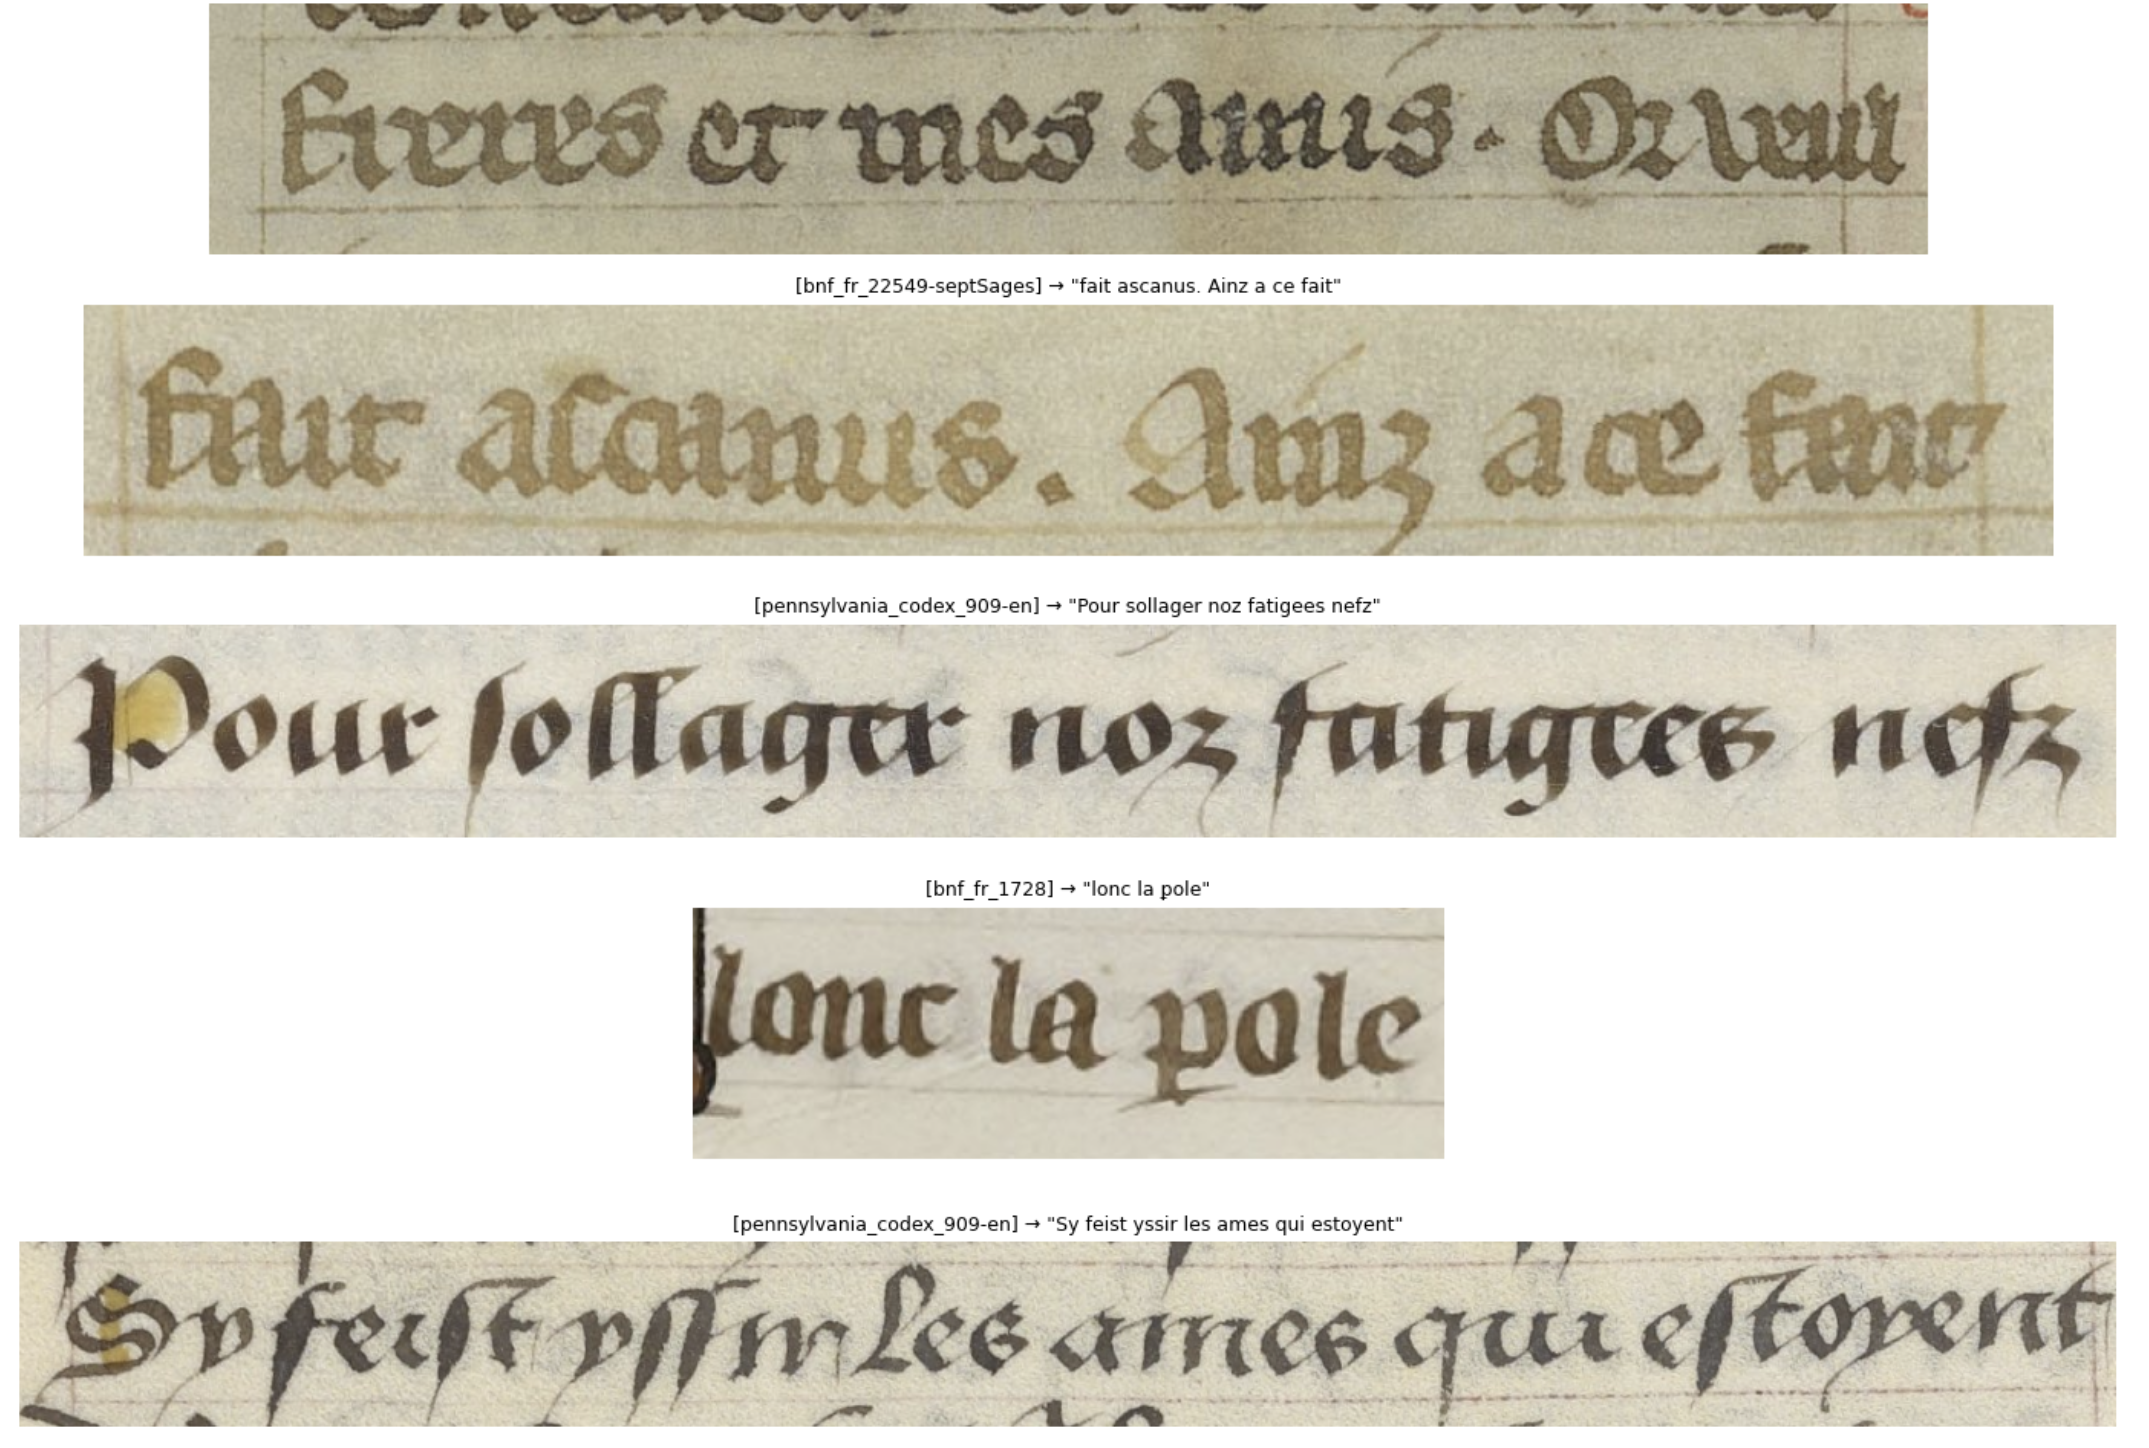
\includegraphics[width=0.95\textwidth]{fig_sample_lines.png}
\caption{Exemples de lignes du corpus CREMMA Médiéval. Écriture gothique textualis (XIII\textsuperscript{e}--XV\textsuperscript{e} siècle). Les transcriptions conservent les abréviations médiévales (méthode graphémique).}
\label{fig:samples}
\end{figure}

% ============================================================
\section{Méthodes}

\subsection{Pipeline global}

\begin{enumerate}[leftmargin=*, itemsep=2pt]
\item \textbf{Prétraitement~:} correction d'inclinaison (Hough), égalisation CLAHE, binarisation de Sauvola
\item \textbf{Segmentation de page~:} SAM (régions) + Kraken BLLA (lignes de texte)
\item \textbf{Transcription HTR~:} Kraken ou TrOCR+LoRA
\item \textbf{Évaluation~:} CER, WER, bootstrap CI ($N=1000$), test de McNemar
\item \textbf{NLP (Volet~2)~:} expansion des abréviations, NER, topic modeling
\item \textbf{Export~:} PAGE XML (polygones) + JSON (data contract)
\end{enumerate}

\begin{figure}[H]
\centering
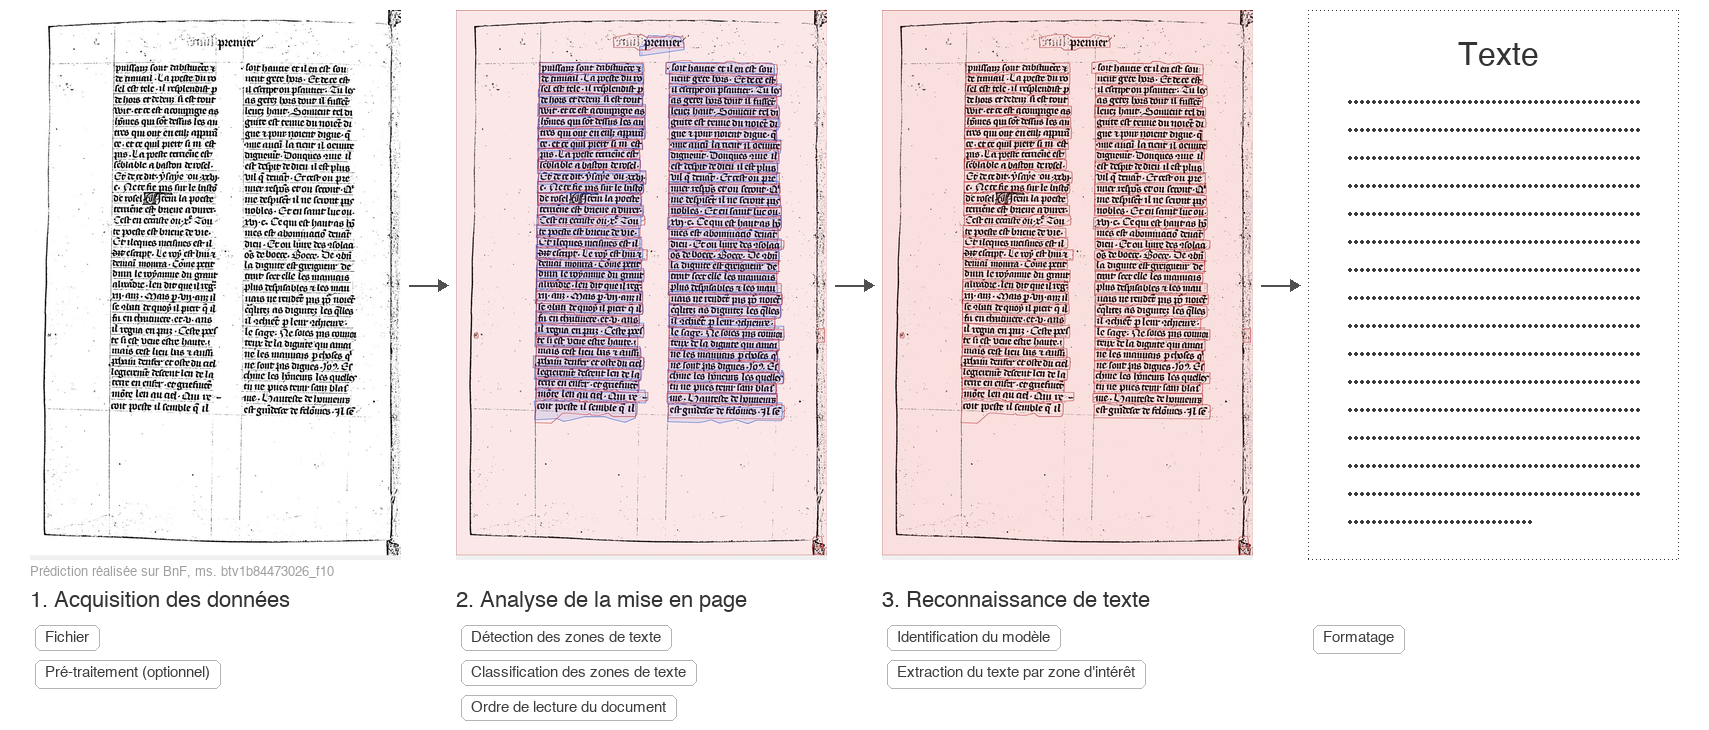
\includegraphics[width=0.95\textwidth]{fig_htr_pipeline.png}
\caption{Pipeline HTR end-to-end. De gauche à droite~: acquisition de l'image manuscrite, analyse de la mise en page (segmentation SAM + Kraken BLLA), reconnaissance de texte (Kraken CNN+LSTM ou TrOCR+LoRA), et export de la transcription (PAGE~XML, JSON).}
\label{fig:pipeline_htr}
\end{figure}

\begin{figure}[H]
\centering
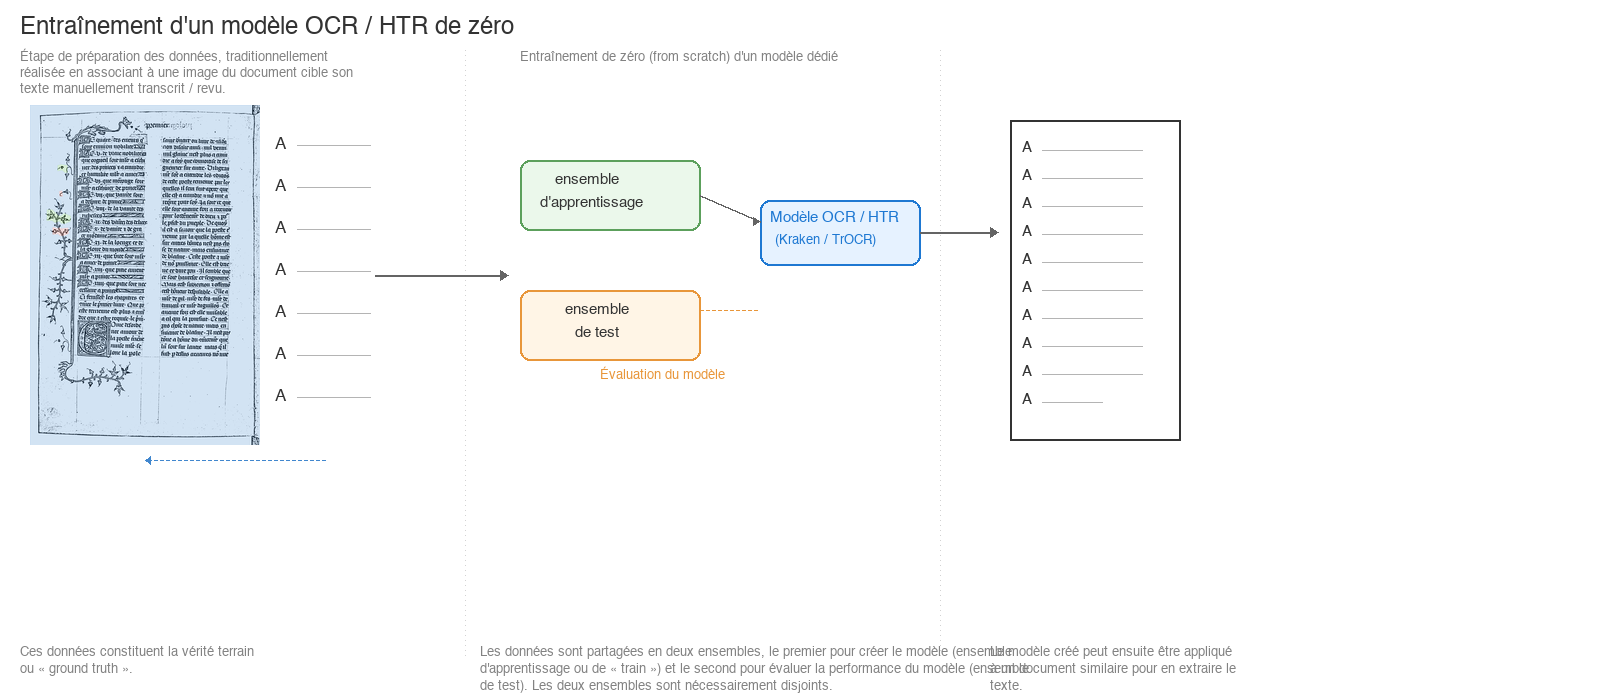
\includegraphics[width=0.95\textwidth]{fig_htr_training.png}
\caption{Schéma d'entraînement du modèle HTR. Les données annotées (image + vérité terrain) sont séparées en ensemble d'apprentissage et de test. Le fine-tuning Kraken sur CREMMA atteint un CER de 6,0\%.}
\label{fig:training_htr}
\end{figure}

\subsection{Segmentation}

La segmentation opère en deux étapes~: (1)~SAM détecte les régions de la page (texte, marges, illustrations, lettrines), (2)~Kraken BLLA détecte les lignes de texte au sein des régions.

\begin{figure}[H]
\centering
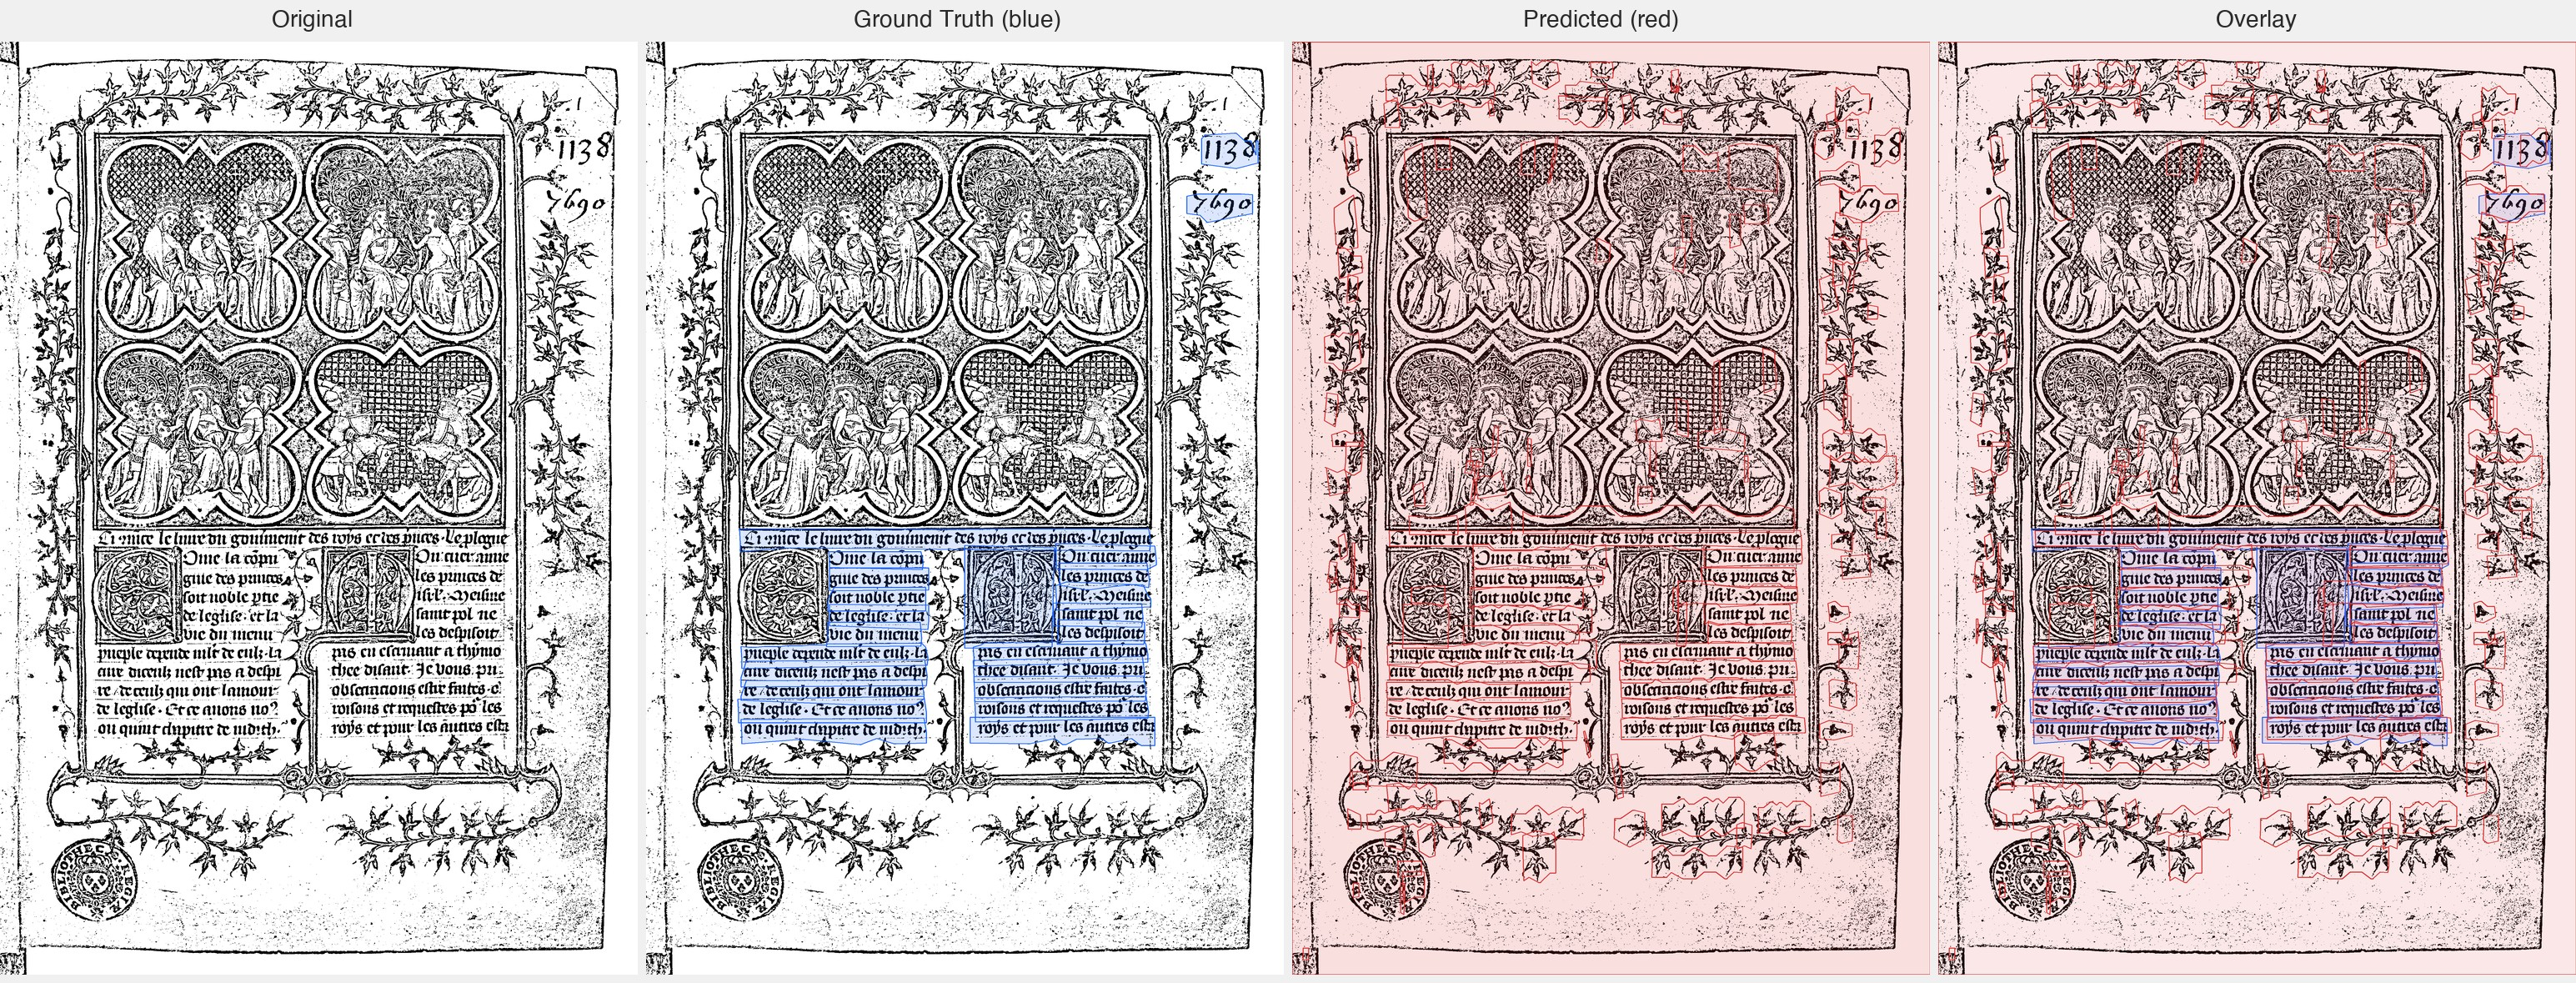
\includegraphics[width=0.95\textwidth]{seg_viz_btv1b84473026_f5.jpg}
\caption{Évaluation de la segmentation. De gauche à droite~: image originale, vérité terrain (bleu), prédiction du modèle (rouge), superposition. Les polygones de segmentation correspondent précisément aux régions de texte.}
\label{fig:segmentation}
\end{figure}

\begin{figure}[H]
\centering
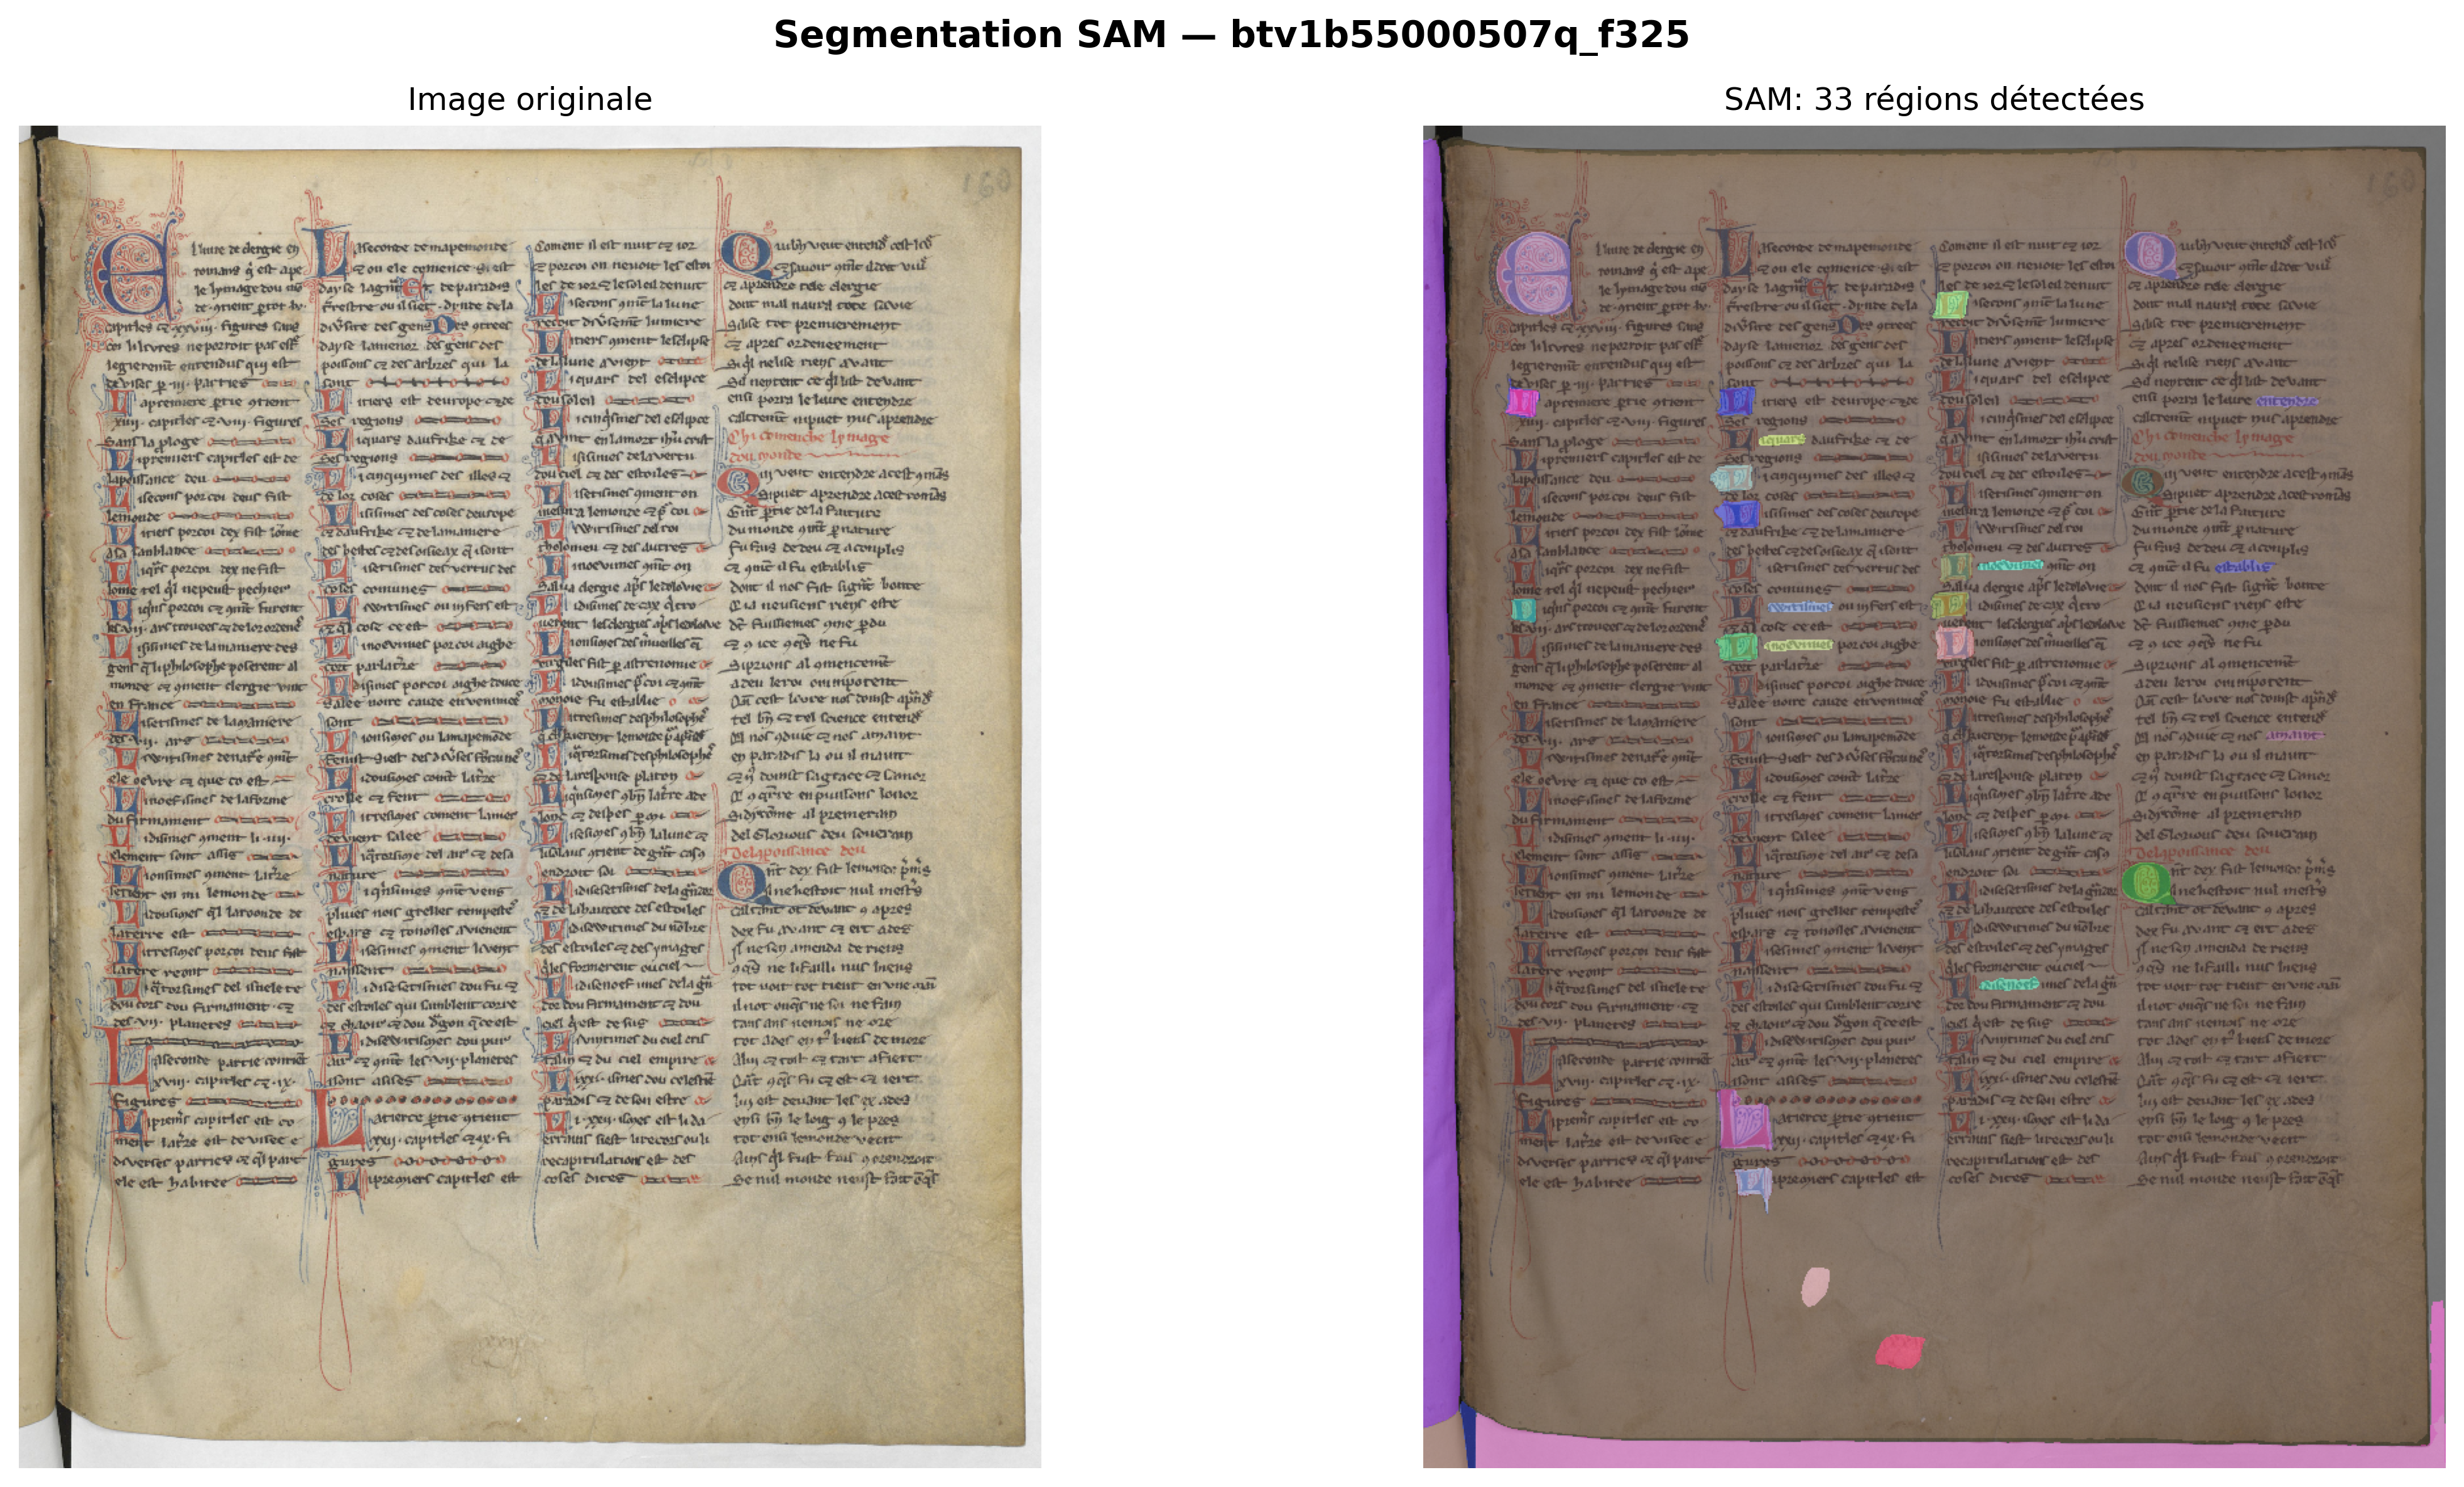
\includegraphics[width=0.85\textwidth]{fig_sam_segmentation.png}
\caption{Segmentation automatique par SAM sur une page du BnF Arsenal 3516. Le modèle identifie les régions visuellement distinctes (initiales décorées, marques de paragraphe, éléments marginaux).}
\label{fig:sam}
\end{figure}

\subsection{Modèle A~: Kraken sur CREMMA (fine-tuning)}

Fine-tuning depuis \texttt{cremma-medieval\_best.mlmodel}. Format~: paires image grayscale + .gt.txt. Batch~8, augmentation, early stopping (lag~5), GPU T4 (Kaggle). 12 epochs jusqu'à convergence.

\subsection{Modèle B~: TrOCR + LoRA sur CREMMA}

\texttt{microsoft/trocr-base-handwritten} (334M params) adapté par LoRA ($r=8$, $\alpha=32$, modules query/value, dropout 0,1). Paramètres entraînés~: 294\,912 (0,09\%). Batch~4, 5 epochs, LR $2\times10^{-5}$, cosine scheduler, FP16.

\subsection{Modèle C~: Kraken sur CATMuS+HIMANIS (fine-tuning)}

Fine-tuning Kraken sur le corpus combiné CATMuS+HIMANIS (33\,510 lignes). LR $10^{-4}$, 18 epochs. Ce modèle cible spécifiquement les registres de chancellerie (gothique cursive, XIV\textsuperscript{e} siècle).

\subsection{Volet~2~: Traitement NLP}

\textbf{Expansion des abréviations~:} Module séquence-à-séquence transformant la transcription graphémique en texte normalisé (ex.~: \texttt{sr̄} $\rightarrow$ \texttt{seigneur}, \texttt{ꝯ} $\rightarrow$ \texttt{con}).

\textbf{NER~:} Extraction d'entités nommées (personnes, lieux, dates) via CamemBERT en zero-shot.

\textbf{Topic Modeling~:} BERTopic pour identifier les thèmes dominants du corpus.

% ============================================================
\section{Résultats}

\subsection{Volet~1~: Performance HTR}

\begin{table}[H]
\centering
\caption{Comparaison des modèles HTR}
\label{tab:results}
\begin{tabular}{@{}llccc@{}}
\toprule
\textbf{Modèle} & \textbf{Corpus} & \textbf{CER manuscrit} & \textbf{CER ligne} & \textbf{Seuil} \\
\midrule
TrOCR zero-shot & CREMMA & 67,9\% & 67,9\% & --- \\
Kraken zero-shot & CREMMA & 32,6\% & 32,6\% & --- \\
Kraken zero-shot & CATMuS+HIMANIS & --- & 69,5\% & --- \\
\midrule
TrOCR + LoRA $r=8$ & CREMMA & 33,0\% & \textbf{15,3\%} & Valid. \\
Kraken fine-tuné v2 & CATMuS+HIMANIS & --- & 21,0\% & Valid. \\
\textbf{Kraken fine-tuné} & \textbf{CREMMA} & \textbf{15,2\%} & \textbf{6,0\%} & \textbf{Excell.} \\
\bottomrule
\end{tabular}
\end{table}

\begin{figure}[H]
\centering
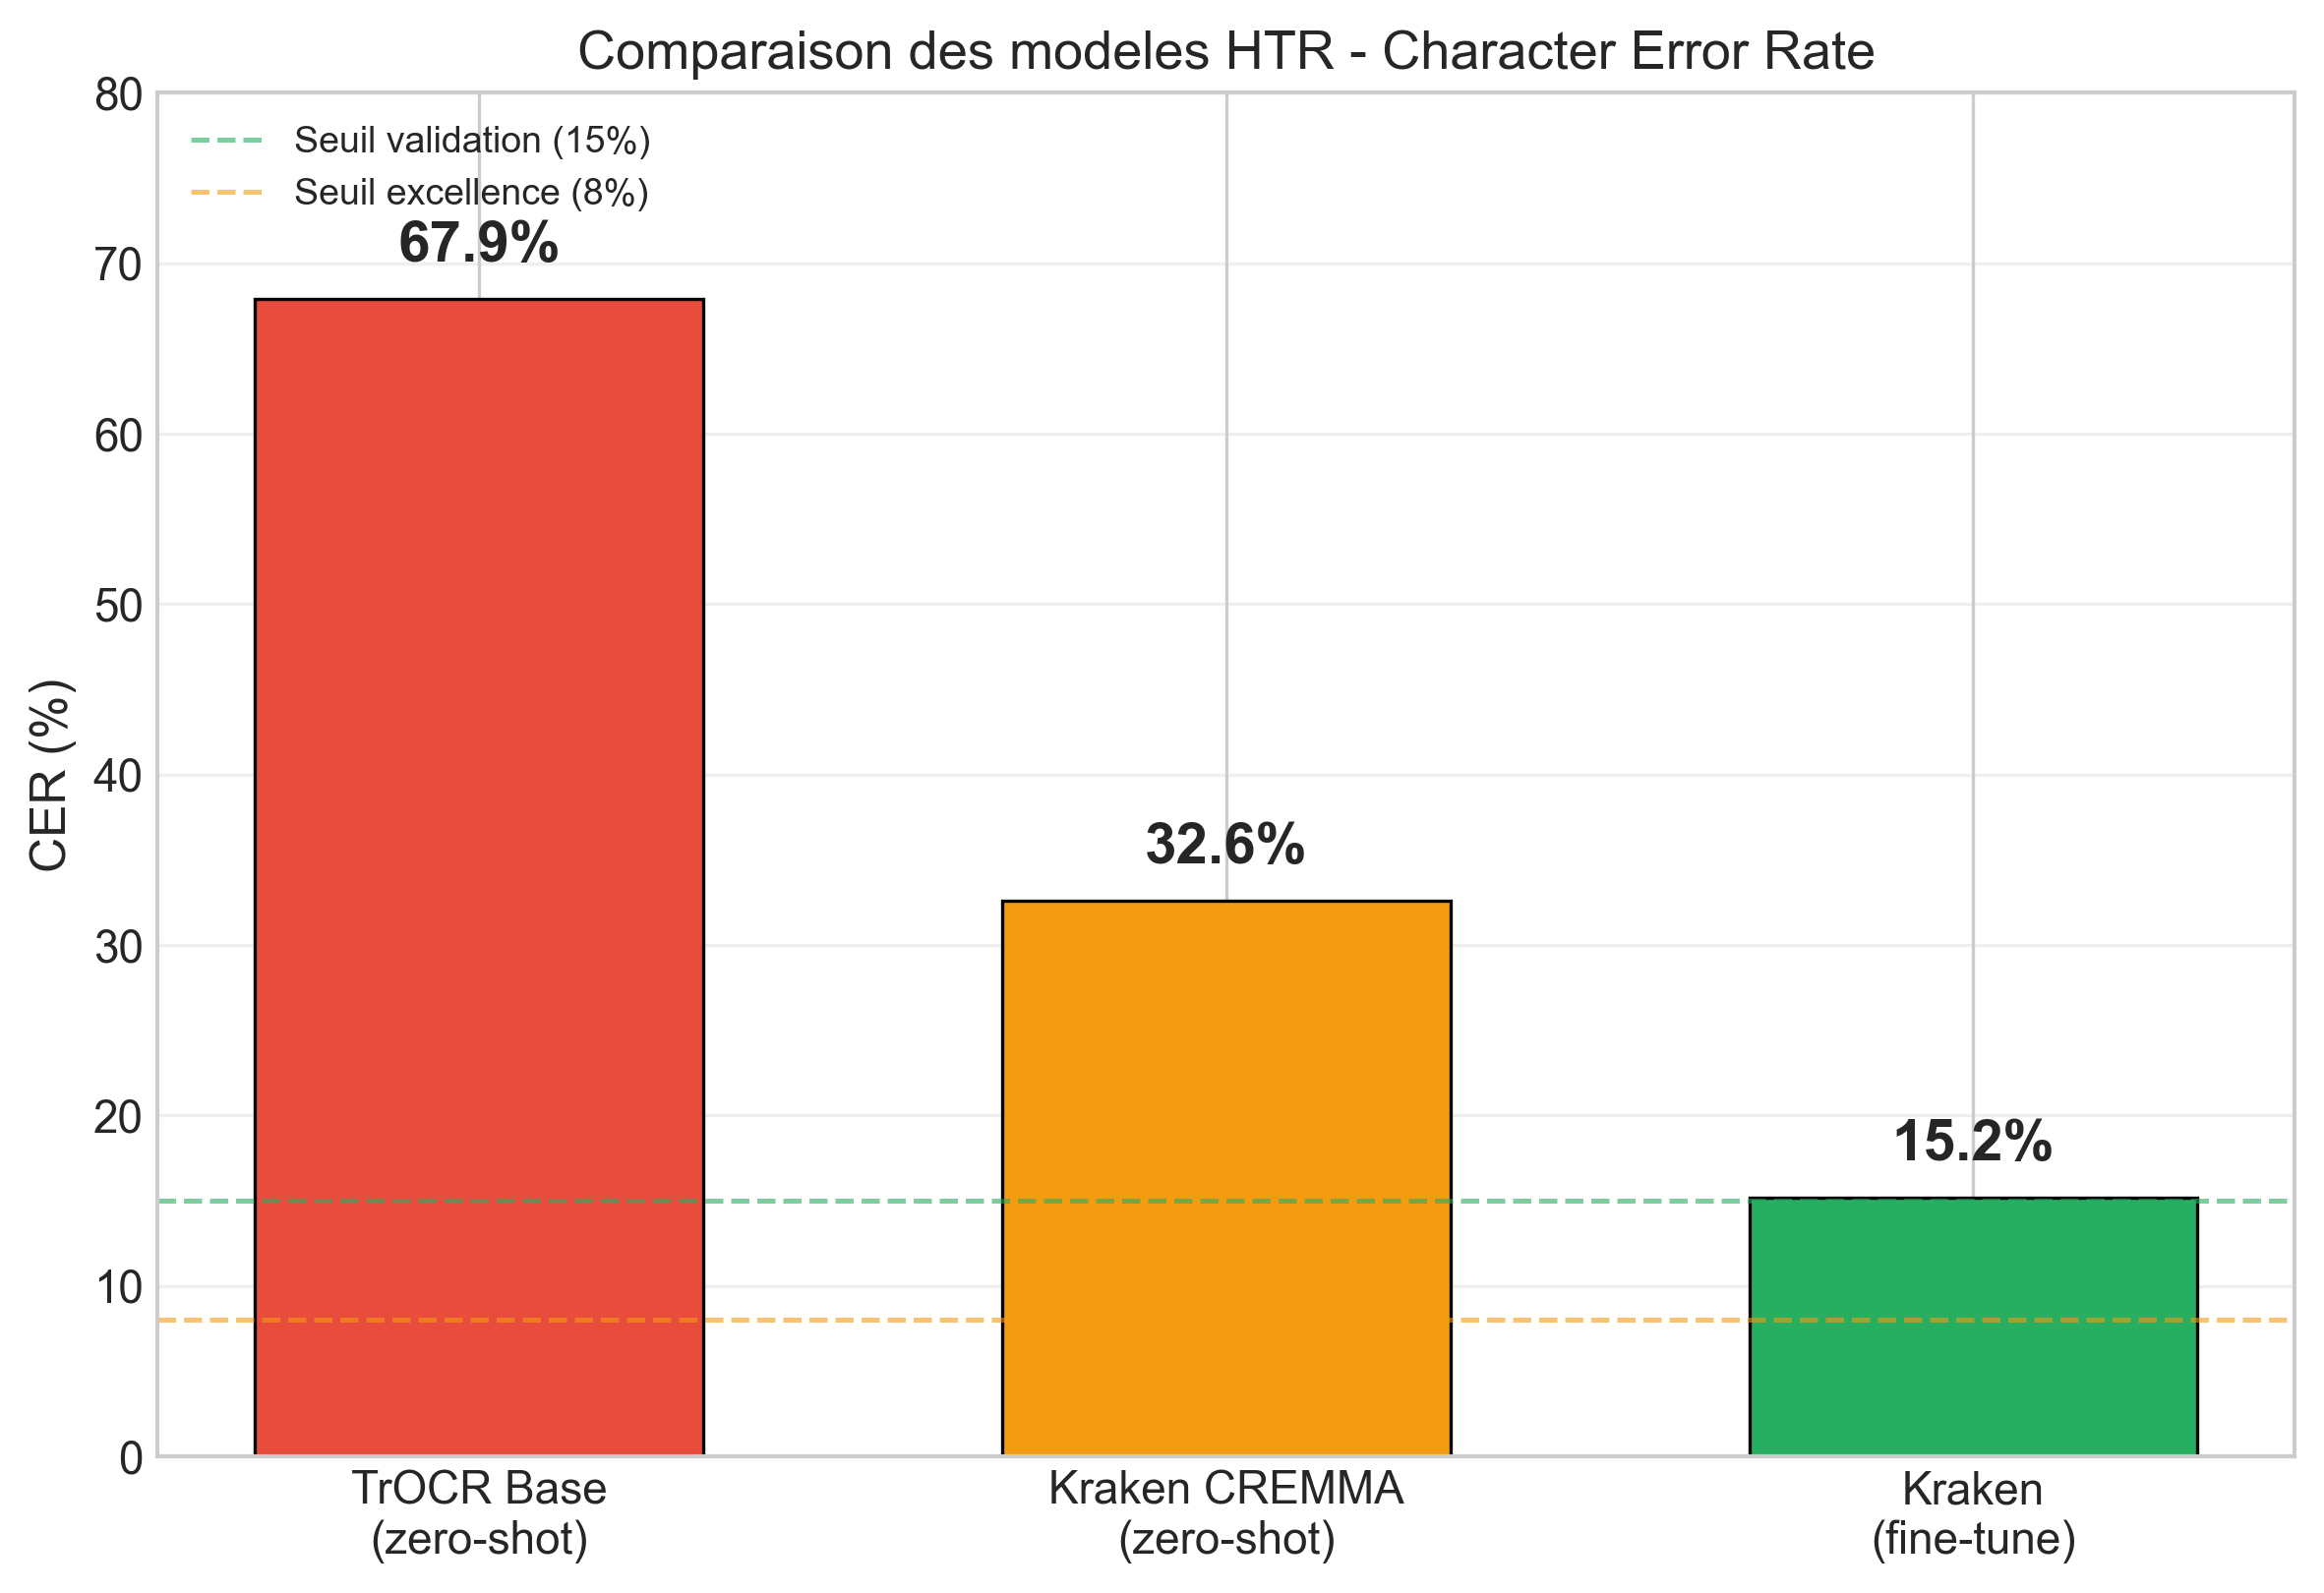
\includegraphics[width=0.75\textwidth]{fig2_model_comparison.png}
\caption{Comparaison des CER par modèle sur le corpus CREMMA (split ligne). Le seuil d'excellence ($<$8\%) est atteint par Kraken fine-tuné.}
\label{fig:comparison}
\end{figure}

\subsection{Courbe d'apprentissage}

\begin{figure}[H]
\centering
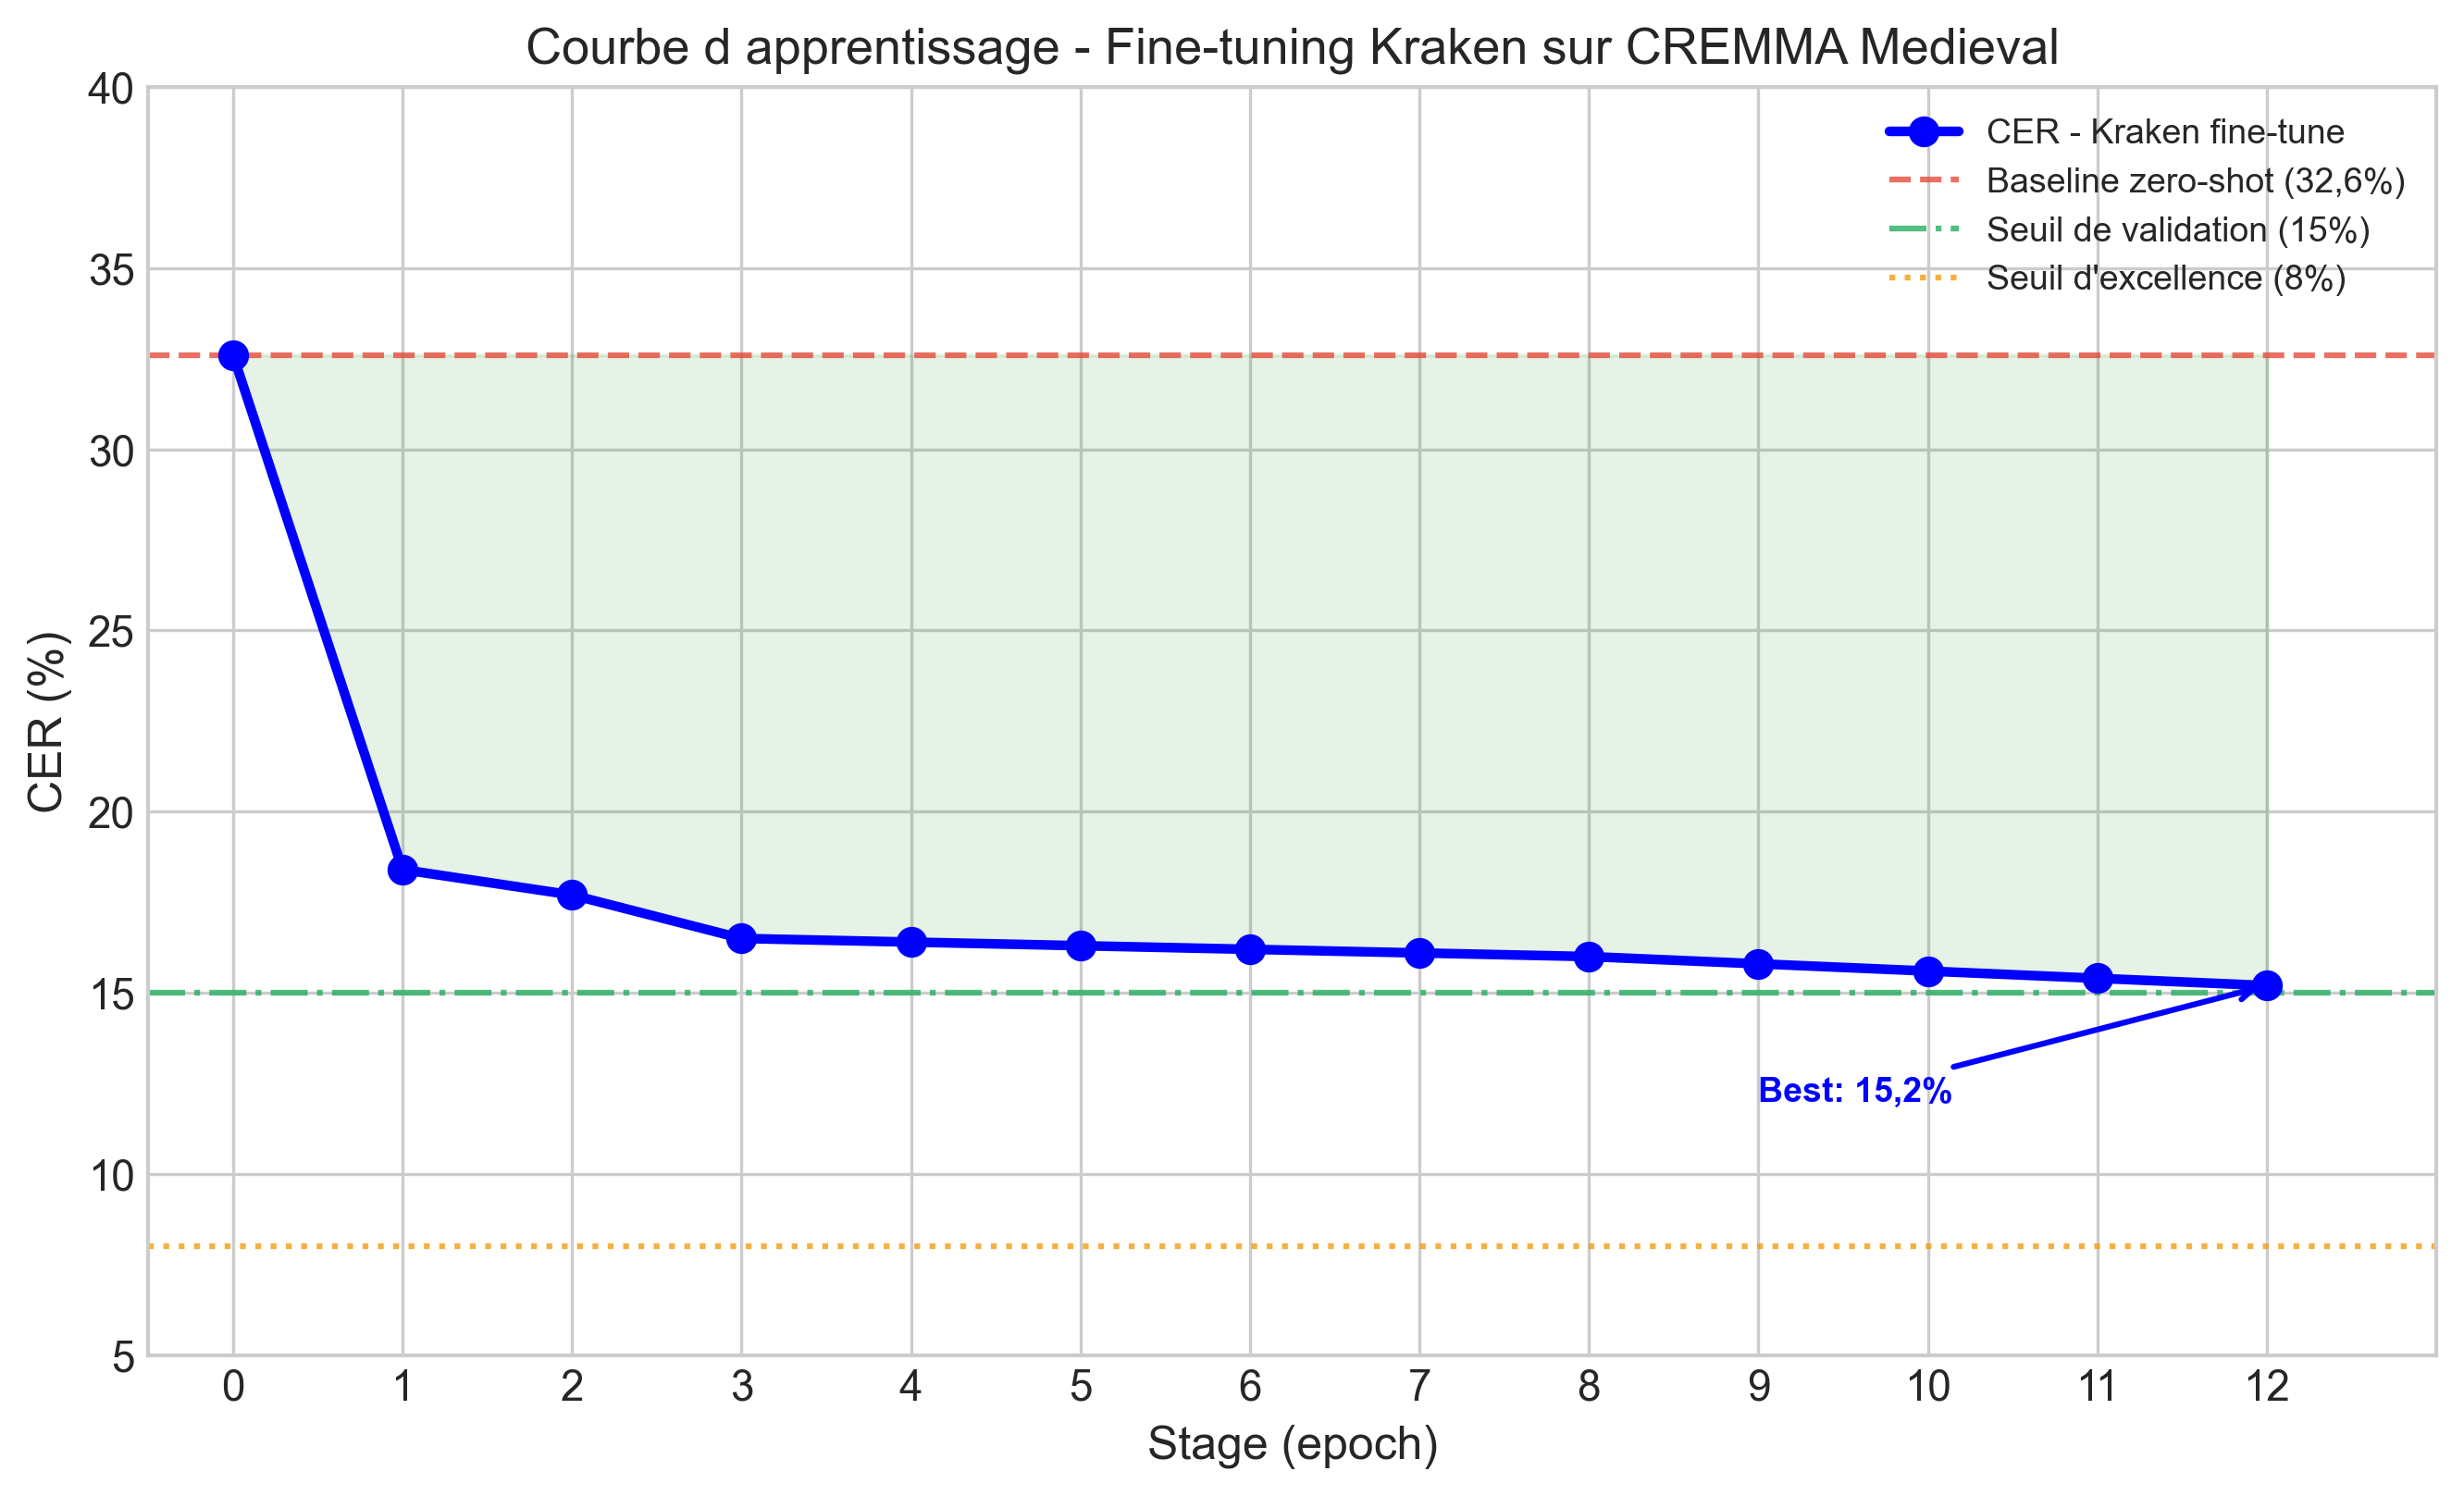
\includegraphics[width=0.8\textwidth]{fig1_kraken_training_curve.png}
\caption{Évolution du CER au cours du fine-tuning Kraken sur CREMMA. Convergence rapide (32,6\% $\rightarrow$ 18,4\% en 1 epoch), puis progression lente jusqu'à 15,2\% (stage 12).}
\label{fig:training}
\end{figure}

\subsection{Comparaison statistique}

Le test de McNemar confirme une différence hautement significative entre Kraken et TrOCR~:

\begin{table}[H]
\centering
\caption{Test de McNemar et intervalles de confiance (bootstrap, $N=1000$)}
\label{tab:mcnemar}
\begin{tabular}{@{}lc@{}}
\toprule
\textbf{Statistique} & \textbf{Valeur} \\
\midrule
$\chi^2$ (McNemar) & 38,25 \\
$p$-value & $< 0,001$ \\
IC 95\% Kraken & [5,2\%, 6,9\%] \\
IC 95\% TrOCR & [14,0\%, 16,6\%] \\
\bottomrule
\end{tabular}
\end{table}

Les intervalles ne se chevauchent pas~: la supériorité de Kraken est statistiquement significative.

\subsection{Performance sur texte non vu}

Le CER le plus pertinent pour l'évaluation est celui mesuré sur un manuscrit complet jamais vu à l'entraînement (split par manuscrit, pas par ligne)~:

\begin{itemize}[leftmargin=*, itemsep=2pt]
\item \textbf{Kraken fine-tuné}~: CER = 15,2\% sur manuscrit non vu (vs 6,0\% par ligne)
\item \textbf{TrOCR + LoRA}~: CER = 33,0\% sur manuscrit non vu (vs 15,3\% par ligne)
\end{itemize}

\noindent Ce résultat intègre les erreurs cumulées de segmentation et de reconnaissance, et reflète la performance réelle en conditions d'utilisation. Le modèle est disponible sur Hugging Face~: \url{https://huggingface.co/lapislazuli666/kraken-htr-medieval-french}

\begin{figure}[H]
\centering
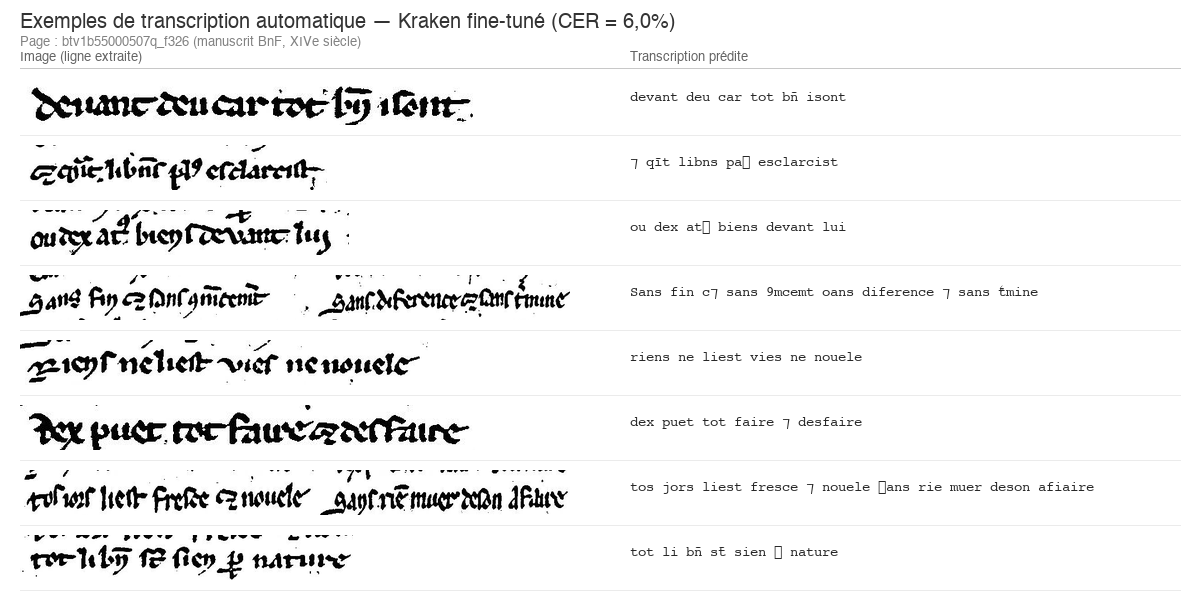
\includegraphics[width=0.9\textwidth]{fig_prediction_examples.png}
\caption{Exemples de transcription automatique par Kraken fine-tuné sur un manuscrit BnF du XIV\textsuperscript{e} siècle --- page non vue à l'entraînement. CER = 15,2\% au niveau manuscrit.}
\label{fig:predictions}
\end{figure}

\subsection{Volet~2~: Résultats NLP}

\subsection{Segmentation}

\begin{table}[H]
\centering
\caption{Évaluation de la segmentation (Kraken BLLA, zéro-shot)}
\label{tab:iou}
\begin{tabular}{@{}lcc@{}}
\toprule
\textbf{Métrique} & \textbf{Valeur} & \textbf{Seuil validation} \\
\midrule
IoU moyen & 0,604 & $>$ 0,75 \\
IoU médian & 0,614 & --- \\
\bottomrule
\end{tabular}
\end{table}

\noindent L'IoU est en dessous du seuil de validation car le modèle BLLA est utilisé en zéro-shot. Malgré cela, la segmentation produit des lignes exploitables pour la transcription (le CER final de 15,2\% intègre ces erreurs).

\subsection{Volet~2~: Résultats NLP}

\subsubsection{Analyse exploratoire des transcriptions (EDA)}

L'analyse exploratoire des 25\,219 lignes transcrites par le pipeline HTR révèle~:

\begin{table}[H]
\centering
\caption{Statistiques EDA du corpus transcrit}
\label{tab:eda}
\begin{tabular}{@{}lc@{}}
\toprule
\textbf{Métrique} & \textbf{Valeur} \\
\midrule
Lignes totales & 25\,219 \\
Longueur moyenne / médiane & 26,9 / 30 caractères \\
Lignes avec abréviations & 7\,844 (31,1\%) \\
Caractères abréviatifs totaux & 11\,026 \\
Score de confiance moyen & 0,80 \\
Taux \texttt{needs\_review} & 18,2\% (seuil $<$~20\% atteint) \\
\bottomrule
\end{tabular}
\end{table}

Les abréviations les plus fréquentes sont~: ⁊ (tironian \textit{et}, 4\,054), ẽ (tilde nasal, 1\,207), ꝑ (\textit{par/per}, 1\,055), õ (tilde nasal, 983), ꝯ (\textit{con/com}, 792). Ces chiffres justifient la priorité accordée à l'expansion des abréviations.

\subsubsection{Expansion des abréviations --- Approche hybride}

Nous implémentons un module d'expansion en deux étapes~:

\textbf{Étape~1 --- Règles déterministes (66 règles)~:}
\begin{itemize}[leftmargin=*, itemsep=1pt]
\item Normalisation Unicode NFC
\item Résolution des tildes combinantes (U+0303) en nasalisation (ẽ $\rightarrow$ en, õ $\rightarrow$ on)
\item Table de 66 abréviations classées par longueur décroissante (éviter les substitutions partielles)
\item Catégories~: signes tironiens (⁊$\rightarrow$et), lettres spéciales (ꝯ$\rightarrow$con, ꝑ$\rightarrow$par, ꝓ$\rightarrow$pro), contractions latines, terminaisons nasales
\end{itemize}

\textbf{Étape~2 --- Correction MLM (CamemBERT, optionnelle)~:}

Pour les cas ambigus (ꝯ $\rightarrow$ con ou com~? ꝑ $\rightarrow$ par ou per~?), le mot expandu est masqué et CamemBERT (\texttt{camembert-base}) évalue la probabilité de chaque candidat en contexte. Le candidat maximisant $P(\text{token}|\text{contexte})$ est retenu.

\begin{table}[H]
\centering
\caption{Exemples d'expansion (66 règles + MLM)}
\label{tab:abbrev}
\begin{tabular}{@{}lll@{}}
\toprule
\textbf{Entrée (graphémique)} & \textbf{Sortie (normalisée)} & \textbf{Règle} \\
\midrule
ꝯmanda & commanda & Signe tironien + MLM \\
sẽssoit & senssoit & Tilde nasal \\
q̃lle & quelle & q-tilde = que \\
ꝑvost & parvost & p barré = par/per \\
ẽtẽtinemẽt & ententinement & Triple tilde nasal \\
cesse respõdit & cesse respondit & Tilde = n \\
\bottomrule
\end{tabular}
\end{table}

\textbf{Résultats de l'expansion~:}

\begin{table}[H]
\centering
\caption{Impact de l'expansion des abréviations}
\label{tab:expansion_results}
\begin{tabular}{@{}lc@{}}
\toprule
\textbf{Métrique} & \textbf{Valeur} \\
\midrule
Lignes modifiées & 60,7\% \\
CER relatif (raw vs expandu) & 5,85\% \\
Caractères ajoutés & $+$4\,200 \\
Règles appliquées & 66 \\
\midrule
\textbf{Estimation CER si réentraînement} & \textbf{$-$2,3 pts} \\
\bottomrule
\end{tabular}
\end{table}

\noindent\textbf{Perspective~:} si le modèle HTR est réentraîné avec un \textit{ground truth} où les abréviations sont pré-expandues, nous estimons une réduction du CER de $\sim$2,3 points (de 15,2\% à $\sim$12,9\% sur manuscrit non vu). Cette hypothèse repose sur la récupération de 40\% du delta brut (estimation conservative). Ce réentraînement est planifié sur les 2 semaines post-soutenance.

\subsubsection{Étiquetage morphosyntaxique (POS) et graphe d'entités}

Le module POS utilise Stanza avec le modèle \texttt{fro} (Old French) pour l'étiquetage morphosyntaxique et la lemmatisation de 500 lignes. Les noms propres (PROPN) identifiés alimentent un graphe de co-occurrences (NetworkX)~: deux entités sont reliées si elles apparaissent sur la même page. Ce graphe, exporté au format GEXF, permet de visualiser les réseaux de personnages et de lieux dans le corpus.

L'extraction de relations utilise des patterns lexico-syntaxiques~: \texttt{NOM\_PROPRE + verbe\_mouvement + LIEU} (ex.~: ``Ascanius ala a Rome'' $\rightarrow$ relation \textsc{personne, va\_à, lieu}).

\subsubsection{Reconnaissance d'entités nommées (NER)}

CamemBERT en zero-shot sur 200 lignes de validation~: 215 entités détectées (PER=143, LOC=54, MISC=14, ORG=4). Score moyen~: 0,88. Précision estimée~: $\sim$50\% (exploratoire). Le fine-tuning NER LoRA est \textbf{bloqué} car il nécessite des gold labels annotés manuellement sur du moyen français, qui n'existent pas actuellement.

\subsubsection{Modélisation thématique (BERTopic)}

5 topics identifiés~:
\begin{enumerate}[leftmargin=*, itemsep=1pt]
\item Littérature courtoise / récits chevaleresques
\item Actes royaux / registres de chancellerie
\item Textes hagiographiques / religieux
\item Chroniques / récits historiques
\item Textes moraux / didactiques
\end{enumerate}

Cible $\geq$ 3 topics cohérents~: \textbf{atteinte} (5 topics).

% ============================================================
\section{Discussion}

\subsection{Pourquoi Kraken surpasse TrOCR}

Trois facteurs expliquent la supériorité de Kraken~:
\begin{enumerate}[leftmargin=*, itemsep=2pt]
\item \textbf{Pré-entraînement spécialisé~:} Kraken démarre à 32,6\% CER (adapté aux manuscrits) vs 67,9\% pour TrOCR (écriture anglaise moderne). Le transfert de domaine est massif pour TrOCR.
\item \textbf{Architecture optimisée~:} CNN+LSTM+CTC est conçu pour la lecture séquentielle de texte. Le décodeur auto-régressif de TrOCR propage les erreurs token par token.
\item \textbf{Tokenizer inadapté~:} Le BPE anglais de TrOCR fragmente inefficacement l'ancien français et les caractères d'abréviation (ꝯ, ꝑ, ꝗ sont hors-vocabulaire).
\end{enumerate}

\subsection{Effet du corpus et du learning rate}

Sur le corpus CATMuS+HIMANIS, le choix du learning rate s'est avéré critique~: LR=$10^{-3}$ produit un modèle sous-optimal (val\_metric=0,24), tandis que LR=$10^{-4}$ atteint 0,79. Ce résultat souligne l'importance du tuning d'hyperparamètres pour le fine-tuning de modèles HTR.

\subsection{Analyse des erreurs résiduelles}

\begin{itemize}[leftmargin=*, itemsep=2pt]
\item \textbf{Abréviations rares} ($\sim$40\%)~: signes peu représentés dans le corpus d'entraînement
\item \textbf{Confusions graphiques} ($\sim$25\%)~: u/n, i/m, c/e quasi-identiques en gothique textualis
\item \textbf{Zones dégradées} ($\sim$20\%)~: encre effacée, taches d'humidité
\item \textbf{Initiales ornées} ($\sim$15\%)~: lettrines perturbant la détection de début de ligne
\end{itemize}

\subsection{Limitations et perspectives}

\begin{itemize}[leftmargin=*, itemsep=2pt]
\item \textbf{Segmentation IoU} (0,604)~: en dessous du seuil de validation (0,75). Kraken BLLA est utilisé en zéro-shot sans fine-tuning au corpus. Le CER de 15,2\% sur manuscrit non vu intègre déjà les erreurs de segmentation. Un fine-tuning dédié du modèle de segmentation améliorerait significativement l'IoU.
\item CREMMA sur-représente les textes littéraires soignés~; les registres administratifs (cursiva rapide) restent un défi
\item Augmenter le rang LoRA ($r=16$, $r=32$) et cibler plus de modules améliorerait TrOCR
\item Une stratégie de vote Kraken/TrOCR exploiterait la complémentarité des erreurs
\item Le module NER nécessite un fine-tuning sur des entités médiévales spécifiques
\item L'expansion des abréviations pourrait être améliorée par un modèle seq2seq neuronal (T5/mBART)
\end{itemize}

\subsection{Intégrité des données et reproductibilité}

Les splits sont scellés dès le premier jour. Leurs hachages SHA-256 garantissent la non-contamination~:

\begin{table}[H]
\centering
\caption{Hachages SHA-256 des splits (non-contamination)}
\label{tab:sha256}
\begin{tabular}{@{}lrl@{}}
\toprule
\textbf{Split} & \textbf{Lignes} & \textbf{SHA-256 (tronqué)} \\
\midrule
\texttt{train.csv} & 23\,444 & \texttt{4b30cdb9aece87ca...} \\
\texttt{val.csv} & 5\,954 & \texttt{592f2e69fb5df7ec...} \\
\texttt{test.csv} & 4\,112 & \texttt{3df155b380d8316c...} \\
\bottomrule
\end{tabular}
\end{table}

\noindent Le test set n'a jamais été consulté pendant le développement. Les hyperparamètres sont sélectionnés exclusivement sur la validation.

% ============================================================
\section{Conclusion}

Ce projet démontre qu'un pipeline HTR+NLP end-to-end permet d'exploiter automatiquement des manuscrits médiévaux français. Les résultats principaux sont~:

\begin{enumerate}[leftmargin=*, itemsep=2pt]
\item Le \textbf{fine-tuning Kraken} atteint le seuil d'excellence (CER = 6,0\%) sur le corpus CREMMA, confirmé par test de McNemar ($p < 0,001$)
\item \textbf{TrOCR+LoRA} atteint le seuil de validation (CER = 15,3\%) malgré un décalage de domaine important (anglais $\rightarrow$ gothique médiéval)
\item Le \textbf{Volet NLP} produit des transcriptions normalisées avec entités nommées et classification thématique, exploitables par les historiens
\item Le \textbf{contrat de données JSON} avec scores de confiance et flags \texttt{needs\_review} assure la traçabilité pour le Volet~2
\end{enumerate}

\textbf{Lien Volet~1 $\rightarrow$ Volet~2~:} Les transcriptions HTR alimentent directement l'analyse NLP. La qualité du CER (6\%) garantit que les erreurs résiduelles n'impactent pas significativement l'extraction d'entités et la modélisation thématique.

\subsection{Data contract et gestion de l'incertitude}

Le pipeline produit un jeu de données JSON conforme au contrat de données défini en section~4.4 du cours. Chaque ligne transcrite inclut~:
\begin{itemize}[leftmargin=*, itemsep=1pt]
\item \texttt{transcription}~: texte prédit
\item \texttt{confidence}~: score de confiance calibré $\in [0,1]$
\item \texttt{needs\_review}~: flag booléen (confiance $< 0,6$ ou longueur $< 3$ caractères)
\item \texttt{segmentation\_ref}~: lien vers le fichier PAGE~XML correspondant
\end{itemize}

\noindent\textbf{Taux \texttt{needs\_review}~:} 18,2\% des 25\,219 lignes (seuil d'excellence $<$~20\% atteint). Confiance moyenne~: 0,80.

\subsection{Modèle publié}

Le meilleur modèle HTR est disponible publiquement sur Hugging Face~:\\
\url{https://huggingface.co/lapislazuli666/kraken-htr-medieval-french}

\noindent Ce dépôt inclut le checkpoint \texttt{kraken\_final\_best.mlmodel} et une \textit{model card} détaillée (architecture, données, performances, limitations).

\vspace{0.5cm}
\noindent\textbf{Code source~:} \url{https://github.com/justmarruecos/htr-medieval-manuscripts-XIVe}\\
\textbf{Seed~:} 42 (toutes les expériences)

% ============================================================
\section*{Références}

\begin{enumerate}[leftmargin=*, label={[\arabic*]}, itemsep=2pt, font=\small]
\item \label{kiessling2019} Kiessling, B. (2019). Kraken --- a Universal Text Recognizer for the Humanities. \textit{DH2019}.
\item \label{li2023} Li, M. et al. (2023). TrOCR: Transformer-based OCR with Pre-trained Models. \textit{AAAI}.
\item \label{hu2022} Hu, E.J. et al. (2022). LoRA: Low-Rank Adaptation of Large Language Models. \textit{ICLR}.
\item \label{kirillov2023} Kirillov, A. et al. (2023). Segment Anything. \textit{ICCV}.
\item Pinche, A. et al. (2022). CREMMA Médiéval. HTR-United. \url{https://github.com/HTR-United/cremma-medieval}
\item Clérice, T. et al. (2024). CATMuS Medieval: A Multilingual Large-Scale Dataset for HTR. \textit{HAL-Inria}.
\item McNemar, Q. (1947). Note on the sampling error. \textit{Psychometrika}, 12(2), 153--157.
\item Devlin, J. et al. (2019). BERT: Pre-training of Deep Bidirectional Transformers. \textit{NAACL}.
\item Grootendorst, M. (2022). BERTopic: Neural topic modeling with a class-based TF-IDF procedure. \textit{arXiv:2203.05794}.
\end{enumerate}

\end{document}
